\documentclass[12pt]{report} % Default font size is 11pt, it can be changed here
\usepackage[a4paper, left=3cm, right=2cm, top=3cm, bottom=2cm]{geometry} % Required to change the page size to A4
\usepackage[utf8]{inputenc} % Required for Brazilian accents - ISO-8859-1 format
\usepackage[square,authoryear]{natbib}
\usepackage[brazil]{babel} % Required for Brazilian hyphenation
\usepackage[T1]{fontenc} % Required for Brazilian hyphenation
\usepackage[brazilian,hyperpageref]{backref}
\usepackage[dvipsnames,svgnames,table,xcdraw]{xcolor}
\usepackage{amsmath}
\usepackage{booktabs}
\usepackage{colortbl}
\usepackage{datagidx}
\usepackage{fancyhdr} 
\usepackage{float} 
\usepackage{framed}
\usepackage{graphicx}
\usepackage{hyperref}
\usepackage{indentfirst}
\usepackage{makeidx}
\usepackage{multicol}
\usepackage{multirow}
\usepackage{ragged2e}
\usepackage{sectsty}
\usepackage{setspace}
\usepackage{titlesec}
\usepackage{tocloft}
\usepackage{wrapfig} 
\usepackage{xcolor}
\usepackage{mathptmx}
\usepackage{subfig}	% required for subfloats (subfigures, subtables...)
\usepackage[labelfont=bf]{caption} %Labels in bold

\usepackage{pdfpages} % requerido para incluir a página pdf com a ficha catalográfica

\usepackage{chngcntr}
\counterwithout{figure}{chapter}
\counterwithout{table}{chapter}

%Data formatada mês, ano
\usepackage[pt-BR]{datetime2}
\DTMlangsetup{showdayofmonth=false}

%\usepackage{algorithm}
\usepackage{amssymb}
\usepackage[noend]{algpseudocode}	% pseudo-codigo
\usepackage[portuguese,ruled,linesnumbered,algochapter,titlenumbered]{algorithm2e}

\makeatletter
\def\BState{\State\hskip-\ALG@thistlm}
\makeatother

%\linespread{1.5} 
\renewcommand {\baselinestretch}{1.5}

\setlength\parindent{1.25cm} 
\renewcommand{\backrefpagesname}{Citado na(s) página(s):~}

\renewcommand{\backref}{}

\definecolor{dark-red}{rgb}{0,0,0} % preto - para adequar ao modelo nortese
\definecolor{dark-blue}{rgb}{0.15,0.15,0.4}
\definecolor{medium-blue}{rgb}{0,0,0.5}
\hypersetup{
	colorlinks, linkcolor={dark-red},
	citecolor={dark-blue}, urlcolor={medium-blue}
}

% Numeracao Pagina
\pagestyle{fancy}
\fancyhf{}
\fancyheadoffset{0cm}
\renewcommand{\headrulewidth}{0pt} 
\renewcommand{\footrulewidth}{0pt}
\fancyhead[R]{\thepage}
\fancypagestyle{plain}{%
	\fancyhf{}%
	\fancyhead[R]{\thepage}%
}

%Capítulos centralizados
\chapterfont{}
\sectionfont{\normalsize \bfseries \flushleft}


% Numeracao capitulos em romano
%\renewcommand{\thechapter}{\Numeric{chapter}}
\titleformat{\chapter}[display] 
{\fontsize{18pt}{\baselineskip}\selectfont\bfseries}{\chaptertitlename\ \thechapter}{2em}{}
\titlespacing*{\chapter}{0pt}{-2em}{2em}

\titleformat{\section}[hang] 
{\fontsize{14pt}{\baselineskip}\selectfont\bfseries}{\thesection}{2em}{}
\titlespacing*{\section}{0pt}{1em}{1em}

\titleformat{\subsection}[hang] 
{\fontsize{14pt}{\baselineskip}\selectfont\bfseries}{\thesubsection}{2em}{}
\titlespacing*{\subsection}{0pt}{1em}{1em}

% centraliza Sumario
\setlength{\cftbeforetoctitleskip}{-2em}
\setlength{\cftaftertoctitleskip}{2em}
\renewcommand{\cfttoctitlefont}{\hfill\large\bfseries} 
\renewcommand{\cftaftertoctitle}{\hfill}
\addto\captionsbrazil{\renewcommand*\contentsname{\fontsize{16pt}{\baselineskip}\selectfont \textbf{SUMÁRIO}}}

% Centraliza Lista de Tabelas
\setlength{\cftbeforelottitleskip}{-2em}
\setlength{\cftafterlottitleskip}{2em}
\addto\captionsbrazil{\renewcommand*\listtablename{\fontsize{16pt}{\baselineskip}\selectfont \textbf{LISTA DE TABELAS}}}
\renewcommand{\cftlottitlefont}{\hfill\bfseries\large} 
\renewcommand{\cftafterlottitle}{\hfill}
\newlength{\mylen}
\renewcommand{\cfttabpresnum}{TABELA\enspace}
\renewcommand{\cfttabaftersnum}{:}
\settowidth{\mylen}{\cfttabpresnum\cfttabaftersnum}
\addtolength{\cfttabnumwidth}{\mylen}

% Centraliza Lista de Figuras
\setlength{\cftbeforeloftitleskip}{-2em}
\setlength{\cftafterloftitleskip}{2em}
\addto\captionsbrazil{\renewcommand*\listfigurename{\fontsize{16pt}{\baselineskip}\selectfont \textbf{LISTA DE FIGURAS}}}
\renewcommand{\cftloftitlefont}{\hfill\bfseries\large} 
\renewcommand{\cftafterloftitle}{\hfill}
\renewcommand{\cftfigpresnum}{FIGURA\enspace}
\renewcommand{\cftfigaftersnum}{:}
\settowidth{\mylen}{\cftfigpresnum\cftfigaftersnum}
\addtolength{\cftfignumwidth}{\mylen}

% Centraliza Lista de Algoritmos
\renewcommand*\listalgorithmcfname{\hfill \fontsize{16pt}{\baselineskip}\selectfont \textbf{LISTA DE ALGORITMOS} \hfill}

\newcolumntype{L}[1]{>{\raggedright\let\newline\\\arraybackslash\hspace{0pt}}m{#1}}
\newcolumntype{C}[1]{>{\centering\let\newline\\\arraybackslash\hspace{0pt}}m{#1}}
\newcolumntype{R}[1]{>{\raggedleft\let\newline\\\arraybackslash\hspace{0pt}}m{#1}}

\newcommand\Tstrut{\rule{0pt}{2.6ex}} % = `top' strut
\newcommand\Bstrut{\rule[-0.9ex]{0pt}{0pt}} % = `bottom' strut
\newcommand{\specialcell}[2][c]{%
	\begin{tabular}[#1]{@{}c@{}}#2\end{tabular}}

\graphicspath{{./figures/}}


%- COMEÇAR A EDITAR A PARTIR DESTA PARTE

\newgidx{acronym}{\hfill \fontsize{16pt}{\baselineskip}\selectfont \textbf{LISTA DE ABREVIAÇÕES} \hfill}
\newgidx{symbol}{\fontsize{16pt}{\baselineskip}\selectfont \textbf{LISTA DE SÍMBOLOS}}

\DTLgidxSetDefaultDB{acronym}
%-----------------------------------------------
% Abreviações
%-----------------------------------------------
\newacro{TSM}{Temperatura da Superfície do Mar}
\newacro{PIRATA}{\textit{Prediction and Research Moored Array in the Tropical Atlantic}}
\newacro{SST}{Sea Surface Temperature}
\newacro{ARIMA}{Modelos Autorregressivos Integrados de Médias Móveis}
\newacro{OSEN}{Oscilação Sul do El Niño}
\newacro{ZCIT}{Zona de Convergência Intertropical}
\newacro{AR}{Modelos Autorregressivos}
\newacro{MA}{Modelos de Médias Móveis}
\newacro{ARMA}{Modelos Autorregressivos de Médias Móveis}
\newacro{MSE}{Erro Médio Quadrático}
\newacro{NMSE}{Erro Médio Quadrático Normalizado}
\newacro{MAPE}{Erro Percentual Absoluto Médio}
\newacro{SMAPE}{Erro Percentual Absoluto Médio Simétrico}
\newacro{ATLAS}{\textit{Autonomous Temperature Line Acquisition System}}
\newacro{H0}{Hipótese Nula}
\newacro{ADF}{\textit{Augmented Dickey-Fuller}}
\newacro{KPSS}{\textit{Kwiatkowski-Phillips-Schmidt-Shin}}
\newacro{AICc}{Critério de Informação de Akaike Corrigido}
\newacro{HP}{Horizonte de Previsão}
\newacro{HYCOM}{\textit{HYbrid Coordinate Ocean Model}}
\newacro{CFSv2}{\textit{The NCEP Climate Forecast System} Versão 2}
\newacro{NCEP}{\textit{National Centers for Environmental Prediction}}
\newacro{SVM}{\textit{Support Vector Machine}}
\newacro{CNPq}{Conselho Nacional de Desenvolvimento Científico e Tecnológico}
\newacro{EM-DAT}{\textit{Emergency Events Database}}
\newacro{FUNCEME}{Fundação Cearense de Meteorologia e Recursos Hídricos}
\newacro{IoT}{Internet das Coisas}

\begin{document}
	%----------------------------------------------------------------------------------------
	%	TITLE PAGE
	%----------------------------------------------------------------------------------------
	\pagenumbering{gobble}% Remove page numbers (and reset to 1)
	\pagenumbering{roman}
	%\begin{titlepage}
	
	\thispagestyle{empty} % sem numeracao
	\newgeometry{left=3cm, right=2cm, top=3cm, bottom=2cm}
	\center % Center everything on the page
	
	\begin{minipage}{\textwidth}
		\begin{center}
			{\bfseries \large CENTRO FEDERAL DE EDUCACAÇÃO TECNOLÓGICA\\ CELSO SUCKOW DA FONSECA}\\[16em]
			{\bfseries \LARGE Avaliação de Agregação Temporal na Previsão da Temperatura de Superfície do Mar do Oceano Atlântico}
		\end{center}
	\end{minipage}\\[6em]
	
	\begin{flushright}
		\begin{minipage}{0.5\textwidth}
			\normalsize
			\raggedleft \normalsize Rebecca Pontes Salles
		\end{minipage}\\[6em]
	\end{flushright}
	
	\begin{flushright}
		\begin{minipage}{0.5\textwidth}
			\raggedleft
			Prof. Orientador:\\
			Eduardo Soares Ogasawara, D.Sc.
		\end{minipage}\\
	\end{flushright}
	\vfill	
	{\bfseries \large Rio de Janeiro,\\
		\today} % Date, change the \today to a set date if you want to be precise
	
	%\end{titlepage}
	\pagebreak
	
	%----------------------------------------------------------------------------------------
	%	FOLHA DE ROSTO
	%----------------------------------------------------------------------------------------
	
	%\begin{titlepage}
	\thispagestyle{empty} % sem numeracao
	\newgeometry{left=3cm, right=2cm, top=3cm, bottom=2cm}
	\center % Center everything on the page
	
	\begin{minipage}{\textwidth}
		\begin{center}
			{\bfseries \large CENTRO FEDERAL DE EDUCACAÇÃO TECNOLÓGICA\\ CELSO SUCKOW DA FONSECA}\\[6em]
			{\bfseries \LARGE Avaliação de Agregação Temporal na Previsão da Temperatura de Superfície do Mar do Oceano Atlântico}\\[6em]% Title of your document
			\raggedleft Rebecca Pontes Salles
		\end{center}
	\end{minipage}\\[6em]
	
	\begin{flushright}
		\begin{minipage}{0.5\textwidth}
			\normalsize
			\raggedleft
			Projeto final apresentado em cumprimento às normas do Departamento de Educação Superior do Centro Federal de Educação Tecnológica Celso Suckow da Fonseca, CEFET/RJ, como parte dos requisitos para obtenção do título de Bacharel em Ciência da Computação.
		\end{minipage}\\[6em]
	\end{flushright}
	
	\begin{flushright}
		\begin{minipage}{0.5\textwidth}
			\raggedleft
			Prof. Orientador: \\
			Eduardo Soares Ogasawara, D.Sc.
		\end{minipage}\\
	\end{flushright}
	\vfill	
	{\bfseries \large Rio de Janeiro,\\
		\today} % Date, change the \today to a set date if you want to be precise
	
	%\end{titlepage}
	\pagebreak
	
	%----------------------------------------------------------------------------------------
	%	Ficha Catalografica
	%----------------------------------------------------------------------------------------
	
	%\pagenumbering{gobble}% Remove page numbers (and reset to 1)
	
	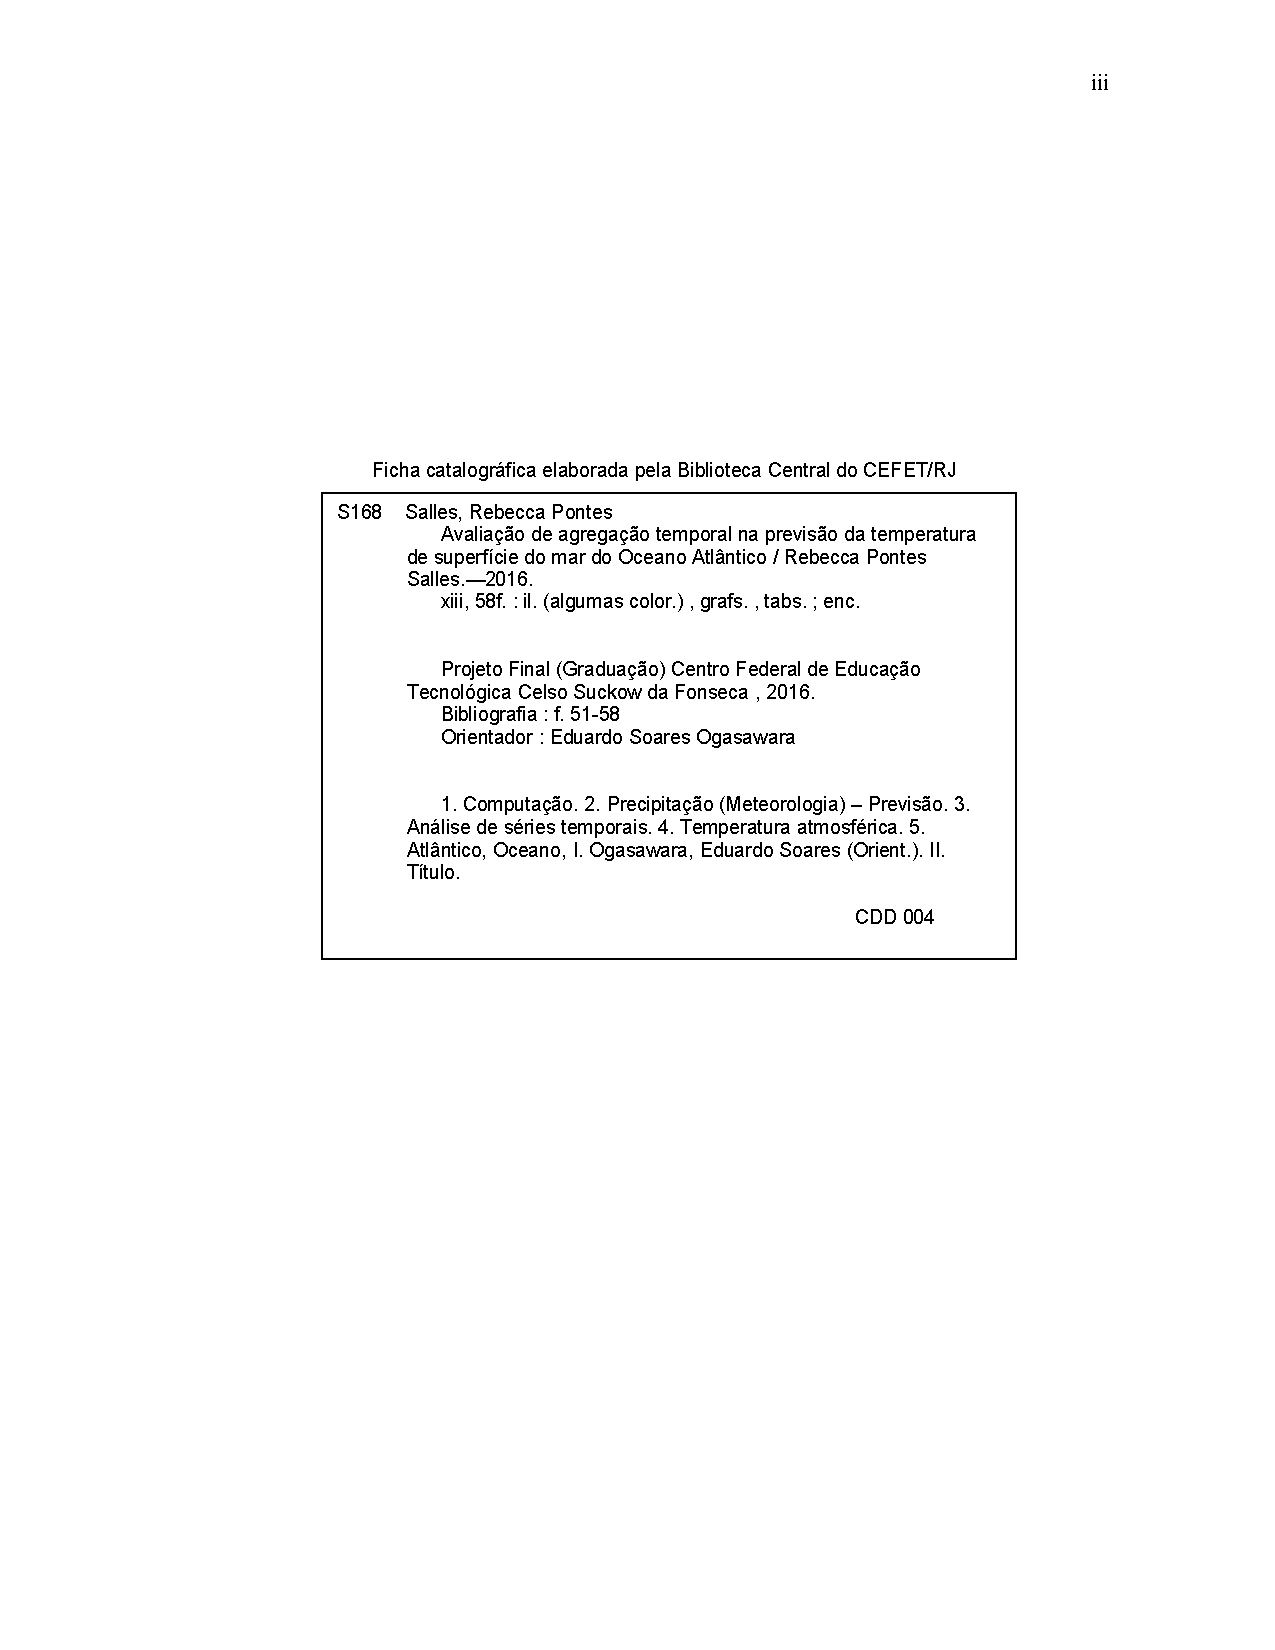
\includepdf{ficha.pdf} % página pdf feita pela biblioteca
	
	\iffalse % COMENTÁRIO
	\center % Center everything on the page
	
	\fbox{%
		\hspace{1cm}
		\parbox{0.6\textwidth}{%
			\footnotesize
			
			Salles, Rebecca Pontes.
			
			\hspace{0.3cm} Avaliação de Agregação Temporal na Previsão da Temperatura de Superfície do Mar do Oceano Atlântico / Rebecca Pontes Salles -- 2016. 
			
			\hspace{0.3cm} \pageref{lastpretextualpage},   \pageref{lastpage}f; enc.
			\singlespacing
			\hspace{0.3cm} Projeto Final (Graduação), Centro Federal de Educação Tecnológica Celso Suckow da Fonseca, 2016. 
			
			\hspace{0.3cm} Bibliografia: f, \pageref{bibpage}--\pageref{bibfinalpage}
			
			\doublespacing
			
			\hspace{0.3cm} \textit{1. Modelos de previsão 2. Séries temporais 3. Agregação temporal 4. Temperatura da superfície do mar 5. Oceano Atlântico I. Título}
		}%
	}
	\fi % FIM DO COMENTÁRIO
	
	\pagebreak
	
	%----------------------------------------------------------------------------------------
	%	Dedicatória
	%----------------------------------------------------------------------------------------
	
	{\fontsize{16pt}{\baselineskip}\selectfont \textbf{DEDICATÓRIA}}
	%\thispagestyle{empty}
	\vspace*{15em}%
	\begin{flushright}
		\begin{minipage}{0.5\textwidth}
			\raggedleft \normalsize A Deus e à minha família amada que me ajudaram, apoiaram e guiaram ao longo de toda a minha vida.
		\end{minipage}\\[1.5cm]
	\end{flushright}
	
	\pagebreak
	
	%----------------------------------------------------------------------------------------
	%	Agradecimentos
	%----------------------------------------------------------------------------------------
	
	{\fontsize{16pt}{\baselineskip}\selectfont \textbf{AGRADECIMENTOS}}
	%\thispagestyle{empty}
	\vspace*{10em}%
	\begin{flushright}
		\begin{minipage}{0.5\textwidth}
			\normalsize
			Agradece-se ao \acr{CNPq} pelo financiamento parcial desta pesquisa.\\
			\\
			Agradece-se também as contribuições de Patricia Mattos que deu início a pesquisas sobre o tema abordado.
		\end{minipage}\\[1.5cm]
	\end{flushright}
	
	\pagebreak
	
	%----------------------------------------------------------------------------------------
	%	Resumo
	%----------------------------------------------------------------------------------------
	
	\begin{center}
		{\fontsize{16pt}{\baselineskip}\selectfont \textbf{RESUMO}}\\[2em]
	\end{center}
	
	\justifying 
	\noindent
	O crescente aumento de congestionamentos no tráfego rodoviário demanda pesquisas relacionadas a mobilidade urbana. Essas pesquisas modelam o problema do tráfego como de trajetória, a partir da análise individualizada de objetos móveis que continuamente transmitem sua geolocalização. Um exemplo disso são os ônibus do Rio de Janeiro. Tais veículos funcionam como sensores de trajetória e produzem grande quantidade de dados. Algumas questões, no entanto, continuam em aberto, como características do transporte público em horários de pico e comportamentos sistêmicos presentes nas diferentes regiões que interfiram na mobilidade da cidade. A agregação espaço-temporal dos dados das trajetórias dos modais urbanos oferece uma visão sumarizada dos dados com potencial para identificação de padrões sistêmicos. Este trabalho visa a aplicar técnicas de identificação de motifs sobre esses dados agregados. Espera-se encontrar padrões que expliquem as diferentes formações e propagações de atrasos, bem como outros fenômenos escondidos sob esse grande volume de dados.
	\\[3em]
	
	\normalsize\noindent
	\textbf{Palavras-chave}: modelos de previsão; séries temporais; agregação temporal; temperatura da superfície do mar; Oceano Atlântico
	
	\pagebreak
	
	%----------------------------------------------------------------------------------------
	%	Abstract
	%----------------------------------------------------------------------------------------
	
	\begin{center}
		{\fontsize{16pt}{\baselineskip}\selectfont \textbf{ABSTRACT}}\\[2em]
	\end{center}
	
	\justifying
	\noindent
	Extreme environmental events such as droughts affect millions of people all around the world. Although it is not possible to prevent this type of event, its prediction under different time horizons enables the mitigation of eventual damages caused by its occurrence. An important variable for identifying occurrences of droughts is the \acr{SST}. In the Tropical Atlantic Ocean, \acr{SST} data are collected and provided by the Prediction and Research Moored Array in the Tropical Atlantic (\acr{PIRATA}) Project, which is an observation network composed of sensor buoys arranged in this region. Sensors of this type, and more generally Internet of Things (\acr{IoT}) sensors, commonly lead to data losses that influence the quality of data sets collected for adjusting prediction models. In this paper, we explore the influence of temporal aggregation in predicting step-ahead \acr{SST} considering different prediction horizons and different sizes for training data sets. We have conducted several experiments using data collected by \acr{PIRATA} Project. Our results point out scenarios for training data sets and prediction horizons indicating whether or not temporal aggregated \acr{SST} time series may be beneficial for prediction.
	\\[3em]
	
	\normalsize\noindent
	\textbf{Keywords}: prediction models; time series; temporal aggregation; sea surface temperature; Atlantic Ocean
	
	
	\pagebreak
	
	%----------------------------------------------------------------------------------------
	%	TABLE OF CONTENTS
	%----------------------------------------------------------------------------------------
	
	\renewcommand{\cftdot}{}
	\tableofcontents % Include a table of contents 
	
	\pagebreak
	
	%----------------------------------------------------------------------------------------
	%	TABLE OF FIGURES
	%----------------------------------------------------------------------------------------
	
	\listoffigures
	
	\pagebreak
	
	%----------------------------------------------------------------------------------------
	%	TABLE OF TABLES
	%----------------------------------------------------------------------------------------
	
	\listoftables
		
	\pagebreak
	
	%----------------------------------------------------------------------------------------
	%	Lista de Abreviações
	%----------------------------------------------------------------------------------------
	
	\printterms[database=acronym,columns=1,prelocation=hfill,style=align]
	
	\label{lastpretextualpage}
	\pagebreak
	
	
	\pagenumbering{arabic}
	\justifying
	
\chapter{Introdução}
\label{sec:introducao}
O aumento da população mundial em áreas urbanas associado ao grande número de veículos presentes nas cidades provocam problemas como congestionamentos, acidentes e poluição \citep{ferreira2013visual,chen2015survey}. No Brasil, o aumento de congestionamentos no tráfego rodoviário de regiões metropolitanas é assunto de preocupação e de constante estudo. Em particular, o Rio de Janeiro desponta como a quarta cidade com pior tráfego no mundo \citep{tomtom2016traffic}. Neste contexto, observa-se a necessidade de intensificação de pesquisas relacionadas à análise de dados do transporte e mobilidade urbana visando a identificação de fatores causadores de congestionamento (gargalos).

Para entender a dinâmica do trânsito urbano e identificar problemas comuns à mobilidade, dados referentes a objetos móveis são coletados principalmente por meio de GPS. No Rio de Janeiro, cada ônibus da frota municipal possui um GPS associado que emite dados referentes à sua geolocalização. Desta forma, cada ônibus corresponde a um objeto móvel e se caracteriza como um sensor de trajetória que coleta e transmite sua localização ao longo do tempo. 

Para compreender estes dados, faz-se valer de técnicas de análise de séries espaço-temporais. As séries espaço-temporais podem ser compostas por observações de objetos móveis ou de objetos permanentes \citep{Frank:2003}. Quando uma das propriedades variantes do objeto é a sua posição, a sequencia de observações do objeto móvel configura o problema de trajetória. Neste contexto, estudam-se, por exemplo, rotas frequentemente observadas pelos objetos e caminhos com propriedades semelhantes \citep{Spaccapietra:2008}. 

No contexto do monitoramento de ônibus, parte dessa análise individualizada já é conhecida, uma vez que os mesmo têm linhas associadas e circulam nas rotas dessas linhas. Algumas perguntas importantes ficam em aberto, como, por exemplo, características do transporte público em horários de pico, ou, também, comportamentos sistêmicos presentes nas diferentes regiões, como padrão de formação e propagação de engarrafamentos e identificação de presença de pontos de interesse, tais como shoppings, escolas e hospitais que possam interferir na mobilidade de uma região da cidade.

Visando cobrir tal lacuna, esta dissertação visa aplicar técnicas de mineração de dados de identificação de \emph{motifs} (padrões não conhecidos) sobre dados agregados de mobilidade urbana. Na agregação espaço-temporal, as informações são agregadas considerando-se um particionamento do tempo (unidade temporal) e do espaço (unidade espacial). Na prática, cada unidade espacial (região) passa a ter uma série espaço-temporal de objeto permanente associada. Esta série é produzida a partir da agregação das informações referentes aos diferentes objetos móveis que percorrem a região na unidade temporal analisada \citep{tao2004spatio}. Intuitivamente, estas séries espaço-temporais agregadas funcionam como sensores virtuais distribuídos. A agregação espaço-temporal favorece uma visão sumarizada dos dados por região. Desta maneira, a partir da análise dos dados de cada unidade espacial e das unidades vizinhas, é possível entender como engarrafamentos se propagam pela cidade. 

Também é possível identificar padrões diferenciados que se repetem em regiões específicas que possam indicar a presença de pontos de interesse. Sendo assim, o desafio consiste em identificar e analisar \emph{motifs} nestas séries agregadas que promovam as respostas aos questionamentos supracitados. Desta forma, o trabalho pretende contribuir ao estabelecer novos algoritmos e técnicas necessárias para identificação e análise desses \emph{motifs} em agregações de séries espaço-temporais de mobilidade urbana. 

Além dessa introdução, o trabalho se divide em mais quatro outras seções. A seção \ref{sec:background} apresenta a revisão da literatura. A seção \ref{sec:trabalhos_relacionados} apresenta os trabalhos relacionados. A proposta propriamente dita é apesentada na seção \ref{sec:proposta}. Finalmente, a seção \ref{sec:estado_atual} apresenta o estado atual do trabalho o planejamento da dissertação. 

\chapter{Preliminares}
\label{sec:background}
Séries espaço-temporais são definidas como sequência de observações que contêm dados sobre o local e momento em que coleta foi feita \citep{cressie2015statistics}. As séries espaço-temporais podem ser caracterizadas como observações de objetos móveis ou objetos permanentes. Os objetos que tem dados de sua localização variantes com o tempo são classificados como móveis. A sequência de observações sobre objetos móveis é classificada como trajetória. A trajetória é o modelo de dados mais aplicado a problemas relacionados ao tráfego \citep{chen2015survey}. Entretanto, estudos que se relacionam mais diretamente com o tema deste trabalho são aqueles em que se agrega informações do objeto \citep{tao2004spatio}, gerando séries espaço-temporais associados a objetos permanentes.

A agregação de dados de objetos móveis pode ser feita de diferentes formas. Os tipos básicos de agregações existentes são Espacial (\emph{S}), Temporal (\emph{T}) e Atributiva ou categórica (\emph{A}). Outros tipos de agregação podem ser feitos a partir da combinação dos tipos básicos, como \emph{$S \times T$}, \emph{$S \times T \times A$} e \emph{$S \times S \times T \times T$} \citep{chen2015survey}. Neste trabalho, a agregação aplicada é a Espaço-Temporal (\emph{$S \times T$}), em que o resultado esperado é composto por séries temporais (T) associadas a pontos geográficos permanentes (S). Tais agregações podem ser interpretadas como sensores virtuais correspondente a região agregada.  

As séries temporais apresentam subsequências que se repetem com frequência. Alguns dos padrões que se repetem não são conhecidos, configurando \emph{motifs} \citep{esling2012time}. A identificação de \emph{motifs} podem ser feita sobre séries temporais univariadas ou multivariadas. Neste trabalho, as séries espaço-temporais obtidas após a agregação \emph{$S \times T$} são multivariadas \citep{wang2016effective} \citep{vahdatpour2009toward}. 


\chapter{Trabalhos Relacionados}
\label{sec:trabalhos_relacionados}
Diversos trabalhos foram desenvolvidos recorrendo à agregações espaço-temporais para lidar com problemas de mobilidade urbana. Normalmente, as agregações feitas nessas pesquisas são baseadas em regiões (AETR), definidas através da projeção de grades sobre a região observada \citep{ferreira2013visual, andrienko2008spatio, adrienko2011spatial,ferreira2013visual}. Nessa classe de trabalhos, pode-se destacar \citet{andrienko2008spatio}, que adotam a agregação espaço-temporal baseada em regiões, enquanto \citet{adrienko2011spatial} adotam dois tipos diferentes de agregação - baseada em tempo e em pontos geográficos permanentes (AETP). A agregação baseada em pontos geográficos permanentes adotada por \citet{adrienko2011spatial} considerou os pontos turísticos da região observada como sensores virtuais.

A identificação de \emph{motifs} em séries espaço-temporais não tem sido explorada na literatura. Em contrapartida, há diversos trabalhos que envolvem identificação de \emph{motifs} sobre séries temporais (IMS) \citep{li2009probabilistic}. \citet{cassisi2013motif}, por exemplo, aplicou a técnica a problemas relacionados à sísmica, \citet{jiang2008finding} ao mercado financeiro e \citet{chi2012face} ao reconhecimento facial. Apesar dos trabalhos listados aplicarem a técnica a problemas reais, a maioria dos trabalhos estudam séries temporais univariadas. 

No contexto de mobilidade urbana, a identificação de \emph{motifs} é feita sobre dados de trajetória (IMT). \citet{schneider2013unravelling} faz uma análise a partir de dados de trajetória individuais. Apesar deste trabalho também visar a identificação de \emph{motifs} em problema de mobilidade urbana, o modelo de dados aplicado é o de séries espaço-temporais associadas a pontos geográficos permanentes. Desta forma, as técnicas de identificação de \emph{motifs} em trajetórias não se adequam ao problema proposto nesse trabalho. 

\begin{table}[!ht]
	\centering
	\caption{Comparação dos trabalhos relacionados}
	\begin{tabular}{ L{6cm} C{1.5cm} C{1.5cm} C{1.5cm} C{1.5cm} }
		\hline\noalign{\smallskip}
		Trabalho & AETR  & AETP & IMS  & IMT \\
		\hline\noalign{\smallskip}
		%\hline\noalign{\smallskip}
		\citet{ferreira2013visual} & X &  &  & \\
		\citet{andrienko2008spatio} & X &  &  & \\
		\citet{adrienko2011spatial} &  & X &  & \\
		\citet{cassisi2013motif} &  &  & X & \\
		\citet{jiang2008finding} &  &  & X & \\
		\citet{chi2012face} &  &  & X & \\
		\citet{schneider2013unravelling} &  &  &  & X \\
		\hline\noalign{\smallskip}
	\end{tabular}
	\label{tbl:sumario}
\end{table}

A tabela \ref{tbl:sumario} apresenta os trabalhos relacionados e as técnicas aplicadas. Áreas mais exploradas são a identificação de \emph{motifs} em séries temporais e a agregação espaço-temporal baseada em região. Não foram observados trabalhos associados a identificação de \emph{motifs} em séries espaço-temporais associadas a objetos permanentes. Observa-se, portanto, uma lacuna para estudo com amplo potencial de exploração.

\chapter{Proposta} 
\label{sec:proposta}
Este trabalho tem como objetivo explorar \emph{motifs} em agregações de séries espaço-temporais de mobilidade urbana.
O trabalho se divide nas fases de pesquisa, implementação e experimentação. Durante a fase de pesquisa, a fundamentação teórica é desenvolvida e aprimorada. A fase de implementação, por sua vez, se divide em três etapas principais: (i) seleção de objetos permanentes (estações), (ii) agregação espaço-temporal e (iii) identificação de \emph{motifs}. A solução implementada é aplicada a uma coleção de dados na fase de experimentação. Posteriormente, faz-se, então, uma análise do significado e relevância dos \emph{motifs} encontrados, confrontando alguns padrões que possam indicar a presença de pontos de interesse com suas reais localizações. 

A seleção de estações tem como objetivo definir objetos permanentes (S) que atuem como sensores virtuais na agregação espaço-temporal. São considerados os dados de localização de todos os pontos de ônibus da cidade do Rio de Janeiro disponíveis no Portal de Dados Abertos da Prefeitura do Rio de Janeiro \citep{datario}. Como algumas áreas tem-se maior presença de pontos de ônibus do que outras, estes pontos foram agrupados utilizando o algoritmo de agrupamento DBSCAN \citep{borah2004improved}. Cada estação passa a ser representada por um \emph{medoid} dos pontos presentes em cada grupo identificado. O objetivo desta técnica é evitar a interferência e sobreposição de pontos muito próximos na agregação espaço-temporal. 

A etapa de agregação espaço-temporal é iniciada com a associação das observações dos objetos móveis a uma estação. Os objetos móveis que atuam como sensores de trajetória são os ônibus do município do Rio de Janeiro e seus os dados também podem ser obtidos no Portal de Dados Abertos da Prefeitura do Rio de Janeiro \citep{datario}. A agregação espaço-temporal considera a velocidade média, quantidade e lista de ônibus e de linhas próximos às estações, considerando-se as unidades de tempo estabelecidas. As agregações calculam estas grandezas tanto no geral quanto por sentido (norte, sul, leste, oeste). Ao fim dessa etapa, são obtidas séries espaço-temporais multivariadas para cada estação. 

Uma vez que as séries espaço-temporais sejam produzidas, aplica-se a identificação de \emph{motifs} sobre essas séries. Em função das propriedades destes dados, pretende-se desenvolver um algoritmo, inspirado em \emph{random projection} \citep{li2009probabilistic}, que introduza restrições espaço-temporais na identificação destes padrões. Estas restrições espaço-temporais visam observar padrões que se propagam ao longo de uma vizinhança. Deste modo, espera-se que sejam emanados padrões capazes de responder as questões de pesquisa previamente mencionadas.  

\chapter{Estado Atual do Trabalho}
\label{sec:estado_atual}

Seguindo o processo de implementação descrito na Seção \ref{sec:proposta}, inicialmente foram definidas as estações (1:Estações) que funcionam como pontos permanentes à agregação espaço-temporal. O primeiro passo é converter os dados geodésicos em um plano cartesiano. Para tanto, foi definido um ponto inicial $P\textsubscript{0}(lat, long)$ referente a menor latitude e longitude do espaço amostral. Em seguida, os pontos de ônibus foram convertidos em pares ordenados, de modo que um ponto de ônibus $P\textsubscript{1}(lat,long)$ seja convertido em $P(x,y)$ tal que $x$ e $y$ são a distância \emph{Harversine} entre $P\textsubscript{2}(lat\textsubscript{P\textsubscript{0}},long\textsubscript{P\textsubscript{1}})$ e $P\textsubscript{0}$ e a distância \emph{Harversine} entre $P\textsubscript{3}(lat\textsubscript{P\textsubscript{1}},long\textsubscript{P\textsubscript{0}})$, respectivamente. Os valores de $x$ e $y$ estão representados na Figura \ref{fig:conversao}.

\begin{figure}[!ht]
	\centering
	\begin{minipage}[t]{0.49\textwidth}
		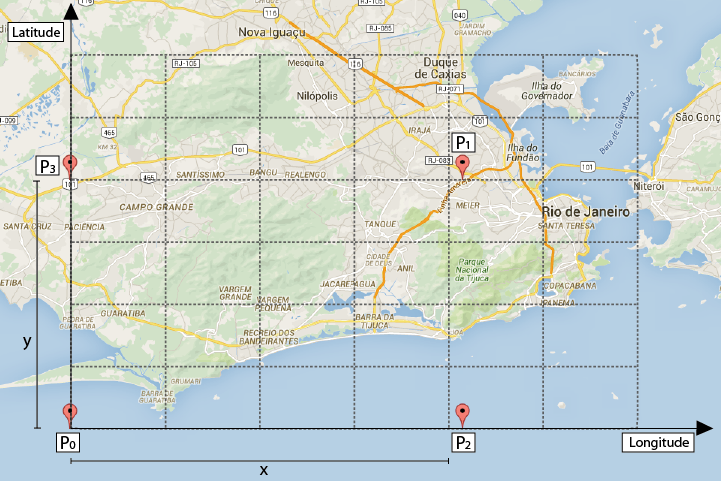
\includegraphics[width=\textwidth]{conversao.png}
		\caption
		{
			Conversão dos dados de localização dos pontos de ônibus.
		}
		\label{fig:conversao}
	\end{minipage}
	\hfill
	\begin{minipage}[t]{0.47\textwidth}
		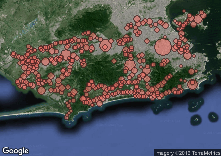
\includegraphics[width=\textwidth]{stations-v3.png}
		\caption
		{
			Estações obtidas aplicando o algoritmo de agrupamento DBSCAN sobre os pontos de ônibus do Rio de Janeiro.
		}
		\label{fig:stacoes}
	\end{minipage}	
\end{figure}

Os pares ordenados obtidos com o processo de conversão dos dados de localização dos pontos de ônibus foram agrupados por DBSCAN, considerando \emph{eps} de 300 metros e o mínimo de um ponto. A partir dos 7020 pontos de ônibus obtidos pelo Portal de Dados Abertos do Rio de Janeiro, foram geradas 307 estações. Na Figura \ref{fig:stacoes}, os marcadores vermelhos indicam as estações obtidas após o agrupamento dos pontos de ônibus. O tamanho do marcador é proporcional a quantidade de pontos que foram agrupados.

As observações de GPS sobre os ônibus da cidade do Rio de Janeiro devem ser associadas às estações, de modo que cada observação seja associada a estação mais próxima. Em seguida, os dados foram agregados às estações, considerando um $\Delta t$ de 1 minuto. No processo de agregação foram obtidos dados referentes a contagem de linhas e de ônibus, velocidade média de ônibus associados a estação e listagem das linhas e dos ônibus associados a estação no momento. Inicialmente, o processo foi executado sobre dados do dia 26 de junho de 2015. Das mais de 4 milhões de observações individuais de ônibus, foram geradas 278.307 observações agregadas.

Além da agregação considerando o $\Delta t = 1 minuto$ , serão realizadas agregações espaço-temporais considerando o $\Delta t = 4 minutos$ e $\Delta t = 8 minutos$. Após o processo de agregação (2:Agr.Temp.), teremos como resultado séries espaço-temporais associadas a pontos permanentes. Com as séries espaço-temporais definidas, o desenvolvimento de algoritmos para identificação de \emph{motifs} (3:Id.Motifs) será realizada. A conclusão prevista para os algoritmos \textit{motifs} é janeiro de 2017, abrindo espaço para experimentação (4:Aval.Exp.) e análise dos resultados obtidos (5:Ana.Result.). 

As pesquisas e a produção textual estão sendo realizada em paralelo às demais etapas. A fundamentação teórica (6:Fund.Teo.) se encontra em fase de desenvolvimento e tem conclusão prevista para setembro de 2016. A solução proposta (7:Metodologia) neste trabalho será descrita de forma mais precisa e detalhada até janeiro de 2017. O experimento e seus resultados serão explorados após a etapa de experimentação, levando em conta a produção de artigo (8:Artigo) associado. 

A defesa da dissertação (9:Defesa) está prevista para setembro de 2017. O cronograma, indicado na tabela \ref{tbl:cronograma}, prevê as etapas abordadas neste trabalho. A tabela indica os meses de previsão de conclusão de cada uma das etapas.

\begin{table}[!ht]
	\centering
	\caption{Cronograma de desenvolvimento da dissertação}
	\begin{tabular}{ L{3cm} C{1cm} C{1cm} C{1cm} C{1cm} C{1cm} C{1cm} C{1cm} C{1cm} C{1cm} }
		\hline\noalign{\smallskip}
		Atividade & jun-jul  & ago-set & out-nov & dez-jan & fev-mar & abr-mai & jun-jul & ago-set \\
		\hline\noalign{\smallskip}
		1:Estações & X & & & & & & & \\
		2:Agr.Temp. & X & X & & & & & & \\
		3:Id.Motifs & & & X & X & & & & \\
		4:Aval.Exp. & & & & X & & & & \\
		5:Ana.Result. & & & & & X & X & & \\
		6:Fund.Teo.& X & X & & & & & & \\
		7:Metodologia & & X & X & X & & & & \\
		8:Artigo & & & & & X & X & X & \\
		9:Defesa & & & & & & & & X \\
		\hline\noalign{\smallskip}
	\end{tabular}
	\label{tbl:cronograma}
\end{table}

\label{bibpage}
\addcontentsline{toc}{section}{Referências Bibliográficas}
\bibliography{references}
\bibliographystyle{apa}
\label{bibfinalpage}


\label{lastpage}\end{document}